\section{Systembeskrivelse}
Der ønskes at udvikle et system, der har til formål at støtte musklerne omkring knæleddet hos ALS-patienter under udførelse af en squat-øvelse. Dette gøres for at aflaste patienterne med henblik på at kunne undgå kørestol i de tidlige stadier af sygdommen. 
Systemet skal kunne opsamle EMG-signaler fra rectus femoris samt en spænding fra påsatte accelerometre på henholdsvis låret samt skinnebenet, for således at kunne beregne vinklen over knæet. Disse signaler skal behandles således, at de kan omsættes til signaler, så en prototype af et exoskelet kan udføre en tilsvarende bevægelse. 
Systemet har yderligere til formål at have mulighed for forstærkning af signalet, så mindre muskelkraft vil kunne udløse den samme bevægelse af knæleddet. 
Systemet skal derudover være sikkert og ikke til gene for brugeren, hvorfor trådløs kommunikation anvendes, hvorved galvanisk adskillelse opnås. Herudover skal systemet være batteridrevet, for at undgå en tilkobling til elnettet. Sikkerheden ses yderligere beskrevet i \autoref{sec:brugersikkerhed}. Derudover gøres systemet kompakt og mobilt ved at være batteridrevet. Hvis batterierne ikke kan levere nok strøm til at virke optimalt, skal dette indikeres ved en blinkende LED på spændingsforsyningen. 

\subsection{Overordnet krav til systemet}  \label{sec:overordnet_krav}
\begin{itemize}
\item Systemet skal registrere muskelaktivitet fra rectus femoris 
\item Systemet skal registrere spænding fra accelerometrene, som omregnes til vinklen over knæet
\item Systemet skal reagere på kroppens bevægelse under en squat-øvelse, således det vil kunne benyttes til en prototype af et exoskelet
\item Systemet skal være sikkert og ikke til gene for brugeren 
\item Systemet skal kunne overføre data trådløst til en computer
\item Systemet skal være batteridrevet
\item Systemet skal kunne indikere, hvis der ikke er strøm nok til at virke optimalt
%\item Systemet skal kunne ende ud i en prototype af et exoskelet
\end{itemize}


\subsection{Blokdiagram} \label{sec:blokdiagram} 
\begin{figure}[H]
\centering
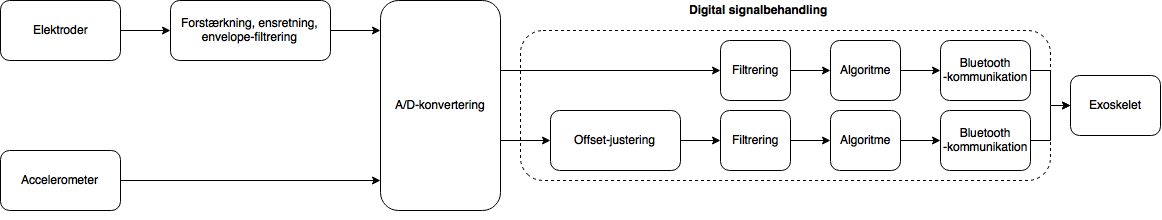
\includegraphics[width=1\textwidth]{figures/blokdiagram.png}
\caption{Systemets opbygning fra sensorer til exoskelet.}
\label{fig:blokdiagram}
\end{figure}

\noindent
I dette projekt er der valgt at udarbejde et kontrolsystem til en prototype, som har til formål at fleksere samt ekstendere knæleddet, ved anvendelse af muskelaktivitet fra rectus femoris. Opbygningen af systemet fremgår af \autoref{fig:blokdiagram}. Der anvendes to sensorer, EMG-elekroder og accelerometre, til at opsamle signaler. 
For at registrere muskelaktivitet anvendes elektroder og en EMG-forstærker, der har til formål at forstærke, filtrere og ensrette muskelsignalet, der opsamles. Hertil anvendes accelerometre ligeledes som et inputsignal.
De opsamlede signaler sendes herefter videre til den digitale del af systemet, hvor en offsetjustering af accelerometer data, filtrering, algoritme samt trådløs kommunikation finder sted. Den digitale del er bestående af et Bluetooth Low Energy Pioneer kit (CY8CKIT-042-BLE), som opfanger signalerne fra EMG-forstærkeren samt accelerometrene. Herefter overføres disse trådløst til en CySmartUSB BLE-dongle sat i en computer, således en visualisering i MATLAB kan forekomme.
